\documentclass[preprint]{article}

%% Load xspace package for proper spacing after commands
\usepackage{xspace}
%% Define the \sys command for the system name
\newcommand{\sys}{SchedCP\xspace}
%% Define the \agent command for the sched-agent name
\newcommand{\agent}{sched-agent\xspace}


\usepackage{neurips_2025}
% \usepackage[final]{neurips_2025}


\usepackage{listings}     % For ASCII-art / code blocks
\usepackage{booktabs}     % Nicer tables
\usepackage{array}        % Column types
\usepackage{tabularx}     % Automatic column width
\usepackage{enumitem}     % Compact lists



\usepackage{comment}

\usepackage[utf8]{inputenc}
\usepackage[T1]{fontenc}
\usepackage{textcomp}
\usepackage[english]{babel} 
\usepackage{url}
\usepackage{graphicx}
\usepackage{subcaption}     % For subfigures


\usepackage{hyperref}       % hyperlinks
\usepackage{amsfonts}       % blackboard math symbols
\usepackage{nicefrac}       % compact symbols for 1/2, etc.
\usepackage{microtype}      % microtypography
\usepackage{xcolor}         % colors




\title{Towards Agentic OS: An LLM Agent Framework for Linux Schedulers}



% \author{%
%   Yusheng Zheng$^{1}$ \quad
%   Yanpeng Hu$^{2}$ \quad
%   Andi Quinn$^{1}$ \\
%   $^{1}$UC Santa Cruz, CA, USA \quad
%   $^{2}$ShanghaiTech University, Shanghai, China \\
%   \texttt{\{yzhen165, aquinn1\}@ucsc.edu, huyp@shanghaitech.edu.cn}
% }
\sloppy
\begin{document}


\maketitle


\begin{abstract}
Operating system schedulers suffer from a fundamental semantic gap, where kernel policies fail to understand application-specific needs, leading to suboptimal performance. We introduce \sys, the first framework that enables fully autonomous Large Language Model (LLM) agents to safely and efficiently optimize Linux schedulers without human involvement. Our core insight is that the challenge is not merely to \emph{apply} a better LLM, but to architect a decoupled control plane that separates the AI's role of semantic reasoning ("what to optimize") from the system's role of execution ("how to observe and act"). Implemented as Model Context Protocol(MCP) server, \sys provides a stable interface with three key services: a Workload Analysis Engine, an evolving Scheduler Policy Repository, and an Execution Verifier that validates all AI-generated code and configure before deployment with static and dynamic analysis. We demonstrate this architecture's power with \agent, a multi-agent system that autonomously analyzes workloads, synthesizes custom eBPF scheduling policies, and deploys them via the sched\_ext infrastructure. Our evaluation shows that SchedCP achieves up to 1.79x performance improvement and 13x cost reduction compared to naive agentic approaches, all while maintaining high success rate. The code will be open-sourced.
\end{abstract}



\maketitle
\section{Introduction}
\label{sec:intro}

Operating system schedulers face a fundamental challenge: kernel policies cannot understand what applications need. This semantic gap leads to suboptimal performance as Linux's EEVDF scheduler~\cite{eevdf2024} applies one-size-fits-all policies to diverse workloads. While sched\_ext~\cite{schedext2024} in Linux 6.12 enables custom extended Berkeley Packet Filter(eBPF) schedulers with safety guarantees through verification, developing them still requires both deep kernel expertise and a good understanding of the workloads.

Prior scheduler optimization approaches using reinforcement learning~\cite{mao2019decima,qiu2020firm} lack semantic understanding of workloads. While LLMs~\cite{openai2023gpt4,anthropic2024claude} and agent frameworks~\cite{autogen,geminicli,claudecode,qian2024chatdev,hong2023metagpt} have shown promise in code generation, naively applying them to scheduler development proves impractical. Our experiments show generating a basic scheduler takes 33 minutes, costs \$6, and often degrades performance. The gap remains: existing methods lack semantic understanding, while LLMs lack the scaffolding for safe, efficient, and reliable systems integration despite previous work exploring LLM for eBPF code generation~\cite{kgent}.

We introduce a decoupled architecture with two components: \sys, a control plane framework providing safe AI-kernel interfaces with profiling, tracing and validation tools, and allow LLM to customize the kernel scheduler with eBPF; and \agent, an autonomous multi-agent system that reasons about workloads and synthesizes or configures existing optimized schedulers. This separation allows \sys\ to provide a generalizable framework for any AI agent, while \agent\ demonstrates semantic workload analysis and policy generation.

\begin{itemize}
    \item \textbf{The \sys\ interface}: A framework that exposes kernel scheduling related features via the Model Context Protocol (MCP), featuring three core services (Workload Analysis Engine, Scheduler Policy Repository, and Execution Verifier) that enable any agent to perform deep semantic analysis of workloads, do AI-driven scheduler optimization without compromising system stability, and learns from experience and improve performance over time.
    \item \textbf{\agent\ multi-agent system}: An autonomous reinforcement learning policy engine that decomposes scheduler optimization into four specialized agents (Observation, Planning, Execution, and Learning), demonstrating how LLMs can bridge the semantic gap between application requirements and kernel scheduling policies.
    \item \textbf{Evaluation}: We demonstrate that \agent\ achieves up to 1.79× performance gains on kernel compilation, 2.11× P99 latency improvement and 1.60× throughput gain on schbench, 20\% average latency reduction for batch workloads, and 13× lower cost compared to naive approaches, while maintaining system stability across diverse workloads.
\end{itemize}

\section{Motivation}
\label{sec:motivation}

We motivate our work by examining the semantic gap problem and practical safety, performance, and cost issues revealed by our experiments. First, a domain knowledge gap exists between developers and users: DevOps engineers configuring Kubernetes lack insight into workload characteristics (latency-sensitive vs. throughput-oriented), resulting in conservative scheduling, while edge and personal device users lack both kernel expertise for doing optimization and understand of the optimization targets of their applications. Second, scheduler development's technical complexity requires mastering kernel programming, limiting innovation to few experts. Third, modern workloads exhibit complex dynamic behavior: web traffic varies by orders of magnitude daily and build system parallelism changes with dependencies. Traditional ML approaches fail here, requiring extensive training data per workload type and unable to generate code. LLMs uniquely bridge these gaps by: (1) understanding natural language and source code semantics without task-specific training, (2) synthesizing correct eBPF scheduler base on the automatically workload characterization, (3) reasoning about performance trade-offs and system constraints, (4) operating in the control plane to generate optimized kernel code with zero runtime overhead. Unlike traditional ML models that would cause unacceptable inference latency in the scheduler hot path, LLMs operate in the control plane to generate optimized code that runs natively in the kernel, ensuring zero runtime overhead while providing 24/7 autonomous optimization capability.


We tested Claude Code\cite{claudecode}, the state of the art LLM agent, with "write a FIFO scheduler in eBPF" from an empty folder, with all permissions and bash access. Of three attempts, only one succeeded. The second attempt produced pseudo-code after 6 minutes trying, and the third generated a scheduler tracer instead after 8 minutes development. The successful generation required 33 minutes, 221 LLM API calls, and 15+ iterations, costing \$6 (vs. 5 minutes typically for an expert developer). The generated code, for some workloads, exhibited poor quality with excessive overhead, performing worse than EEVDF. The agent required root access, could crash the system during testing, and lacked fallback mechanisms, which also raises safety concerns. These experiments reveal three critical challenges: \textbf{Performance}, ensuring AI schedulers outperform existing ones; \textbf{Safety}, preventing crashes, lockups, and starvation while minimizing privileges; and \textbf{Efficiency}, reducing the 33-minute, \$6 generation cost for practical deployment.

\section{The \sys\ Framework Design and Implementation}
\label{sec:schedcp_framework}

\begin{figure}
    \centering
    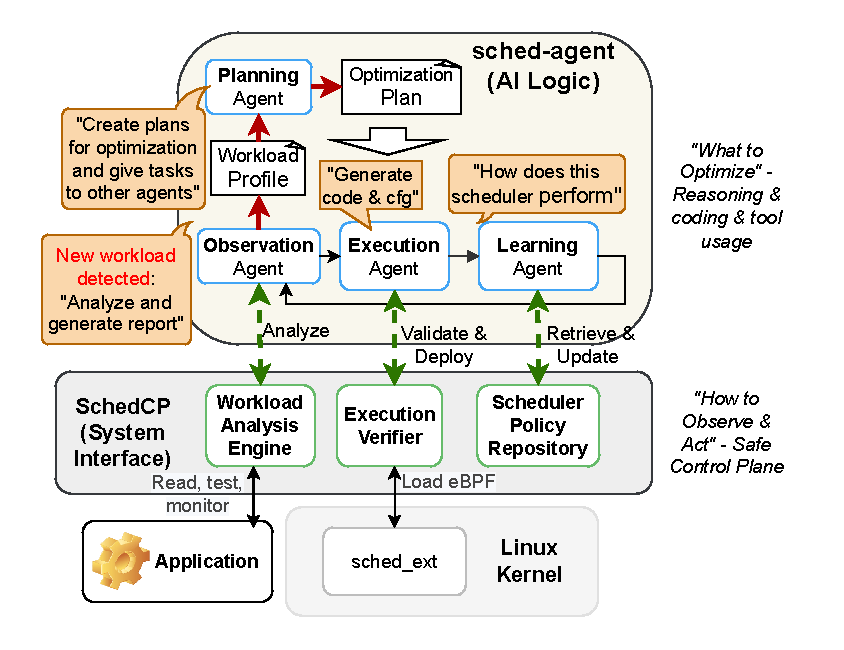
\includegraphics[width=\columnwidth]{sections/img/arch-scheddcp.pdf}
    \caption{
        \textbf{Overall architecture of \sys\ and \agent.} 
        \sys\ (bottom) provides the system interface with three core services: Workload Analysis Engine, Scheduler Policy Repository, and Execution Verifier.
        \agent\ (top) implements the AI logic through four specialized agents (Observation, Planning, Execution, Learning) working in a closed loop. Red lines show initialization when detecting new workloads, black arrows show optimization loops, and green arrows indicate tool usage by agents.
    }
    \label{fig:frameworkarch}
\end{figure}

Our approach to agentic OS optimization separates systems infrastructure from AI logic, as illustrated in Figure~\ref{fig:frameworkarch}. We introduce \sys, a secure control plane that acts as an 'API for OS optimization.' Our research is motivated by the insight that AI agents are fundamentally context engineering systems; like human experts, they need the right tools to gather information and act without being overwhelmed by prohibitive costs or irrelevant data. Therefore, as system researchers, our goal is not to build better AI agents, but to design superior systems and interfaces for them. \sys provides essential tools for any agent to interact with the Linux kernel's scheduler, analogous to how an environment in reinforcement learning provides the state, actions, and rewards for an agent to learn. \sys is implemented in ~4000 lines of Rust and ~6000 lines of python (Include tests).

Four key principles govern \sys's design. First, \textbf{decoupling and role separation} ensures future-proofing by distinguishing ``what to optimize'' (the AI's domain) from ``how to observe and act'' (the system's domain), treating the AI agent as a performance engineer using a stable set of tools. Second, \textbf{safety-first interface design} addresses the inherent risks of autonomous agents with kernel access by treating AI as potentially non-cautious actors and designing defensive interfaces that prevent catastrophic failures by default. Third, \textbf{adaptive context provisioning} addresses LLM agents' constraints from finite context windows and token costs: agents start with minimal summaries and progressively request details as needed. Finally, \textbf{composable tool architecture} follows Unix philosophy by providing atomic tools that let agents construct complex workflows through their reasoning capabilities, enabling novel solution generation rather than constraining them with rigid workflows.

\sys exposes its services to AI agents via the standard Model Context Protocol (MCP)~\cite{anthropic2024mcp}, separating high-level policy orchestration from low-level observation and execution while avoiding granting `root' privileges to the agent. The architecture consists of three primary services.

\textbf{1. Workload Analysis Engine.} This service provides agents with tiered access to system performance data: (1) cost-effective API endpoints delivering pre-processed summaries like CPU load and memory usage, (2) secure sandbox access to basic file reading, application building, standard Linux profiling tools (\texttt{perf}, \texttt{top}) and dynamically attachable eBPF probes for detailed analysis, and (3) a feedback channel that reports post-deployment performance metrics such as percentage change in makespan or latency.

\textbf{2. Scheduler Policy Repository.} This vector database stores executable eBPF scheduler programs with rich metadata: natural language descriptions, target workloads, and historical performance metrics. It provides APIs for semantic search and retrieval, enabling agents to find relevant schedulers or composable code primitives. To support system evolution, it includes endpoints for updating performance metrics and promoting new policies, reducing generation costs by allowing reuse of proven solutions while maintaining a growing library of scheduling strategies.

\textbf{3. Execution Verifier.} This validation pipeline provides multi-stage verification for all AI-generated code and config, beginning with the kernel's standard eBPF verifier to guarantee fundamental memory safety and termination. Because the standard verifier is agnostic to scheduling logic and cannot detect flaws like task starvation or unfairness, our pipeline adds a second layer of scheduler-specific static analysis to check for these correctness and logic bugs. Code that passes both static analysis layers proceeds to dynamic validation, where it is compiled and executed within a secure micro-VM against correctness and performance tests. Upon success, the service issues a signed deployment token for a monitored canary deployment with a circuit breaker to automatically revert to the last known-good scheduler if performance degrades. This also ensures the \agent doesn't need root access to deploy eBPF schedulers.

\section{\agent: A Multi-Agent Framework for OS Optimization}
\label{sec:sched_agents}

Building on \sys, we developed \textbf{\agent}, a multi-agent AI framework implementing in-context reinforcement learning (ICRL)\cite{incontextrl} for scheduler optimization. Using Claude Code's subagent architecture\cite{anthropic2024subagents}, \agent\ decomposes the optimization process into distinct ICRL stages through specialized AI assistants with customized prompts, tools, and separate context windows\cite{anthropic2024multiagent}. The framework integrates with container orchestrators like Kubernetes and Docker to automatically trigger optimization when applications deploy, enabling adaptive strategy refinement based on performance feedback without model retraining.

The framework employs four specialized agents working in concert. The \textbf{Observation Agent} builds comprehensive Workload Profiles by strategically querying the Workload Analysis Engine, starting with high-level summaries then requesting deeper profiling (e.g., \texttt{perf stat}, \texttt{top}) based on findings, synthesizing data into natural language descriptions, performance characteristics, and optimization goals while managing cost-precision tradeoffs. The \textbf{Planning Agent} transforms profiles into optimization strategies by querying the Scheduler Policy Repository, following a decision hierarchy: configuring existing production-ready schedulers, generating patches for partial matches, or composing new schedulers from primitives when no suitable base exists. The \textbf{Execution Agent} manages development, validation and deployment by synthesizing code artifacts, submitting to the Execution Verifier, interpreting results to refine code or fix logic issues, and initiating canary rollouts with circuit breaker protection. The \textbf{Learning Agent} completes the ICRL loop by analyzing deployment outcomes, enabling in-session adaptation and updating the repository with refined metrics, deployment contexts, and documented antipatterns.

Consider kernel compilation as an illustrative example. The Observation Agent analyzes the Linux kernel source tree and \texttt{make -j} process, producing a profile: ``CPU-intensive parallel compilation with short-lived processes, inter-process dependencies, targeting makespan minimization.'' The Planning Agent queries Policy Repository and retrieves \texttt{scx\_rusty} and generates adaptive configurations. After the Execution Agent validates and deploys the patched scheduler, the Learning Agent records the 45\% makespan reduction and contributes the improved scheduler to the repository. This workflow demonstrates \agent's autonomous optimization through iterative refinement.

\section{Evaluation}
\label{sec:evaluation}

% \subsection{Research Questions}

We investigate key research questions to validate the effectiveness and efficiency of \sys: whether it can effectively configure existing schedulers (RQ1) and generate new schedulers for specific workloads (RQ2), what the cost and efficiency of scheduler generation are (RQ3), and how much \agent can continue to improve performance after its initial attempt through iterative refinement (RQ4). We evaluate \sys on two machines: an 86-core Intel Xeon 6787P with 758GB RAM running Linux 6.14, and an 8-core Intel Core Ultra 7 258V with 30GB RAM running Linux 6.13. Agents are built using Claude Code (Opus 4), testing each case three times and averaging results. In all experiments, the agent successfully creates working custom scheduler configurations or eBPF programs.

\textbf{Scheduler Configuration Performance Evaluation}: For kernel compilation with tinyconfig and ``make -j 172'' on 6.14 source code (Figure~\ref{fig:performance-comparison}), \sys achieves 1.63× speedup using scx\_rusty initially, then through iterative refinement selects scx\_layered for 16\% additional gain, reaching 1.79× total improvement over EEVDF. Basic RL approaches~\cite{corbet2025ml} show 1.26x improvement. On schbench~\cite{schbench2016} (Figure~\ref{fig:schbench-comparison}), while initial AI configuration (scx\_bpfland) underperformed with worse P99 latency and lower throughput, three iterations of refinement identified scx\_rusty as superior, achieving 2.11× better P99 latency and 1.60× higher throughput versus EEVDF, demonstrating effective learning from performance feedback.

\begin{figure}[h]
\centering
\begin{minipage}{0.48\textwidth}
    \begin{subfigure}[b]{\textwidth}
        \centering
        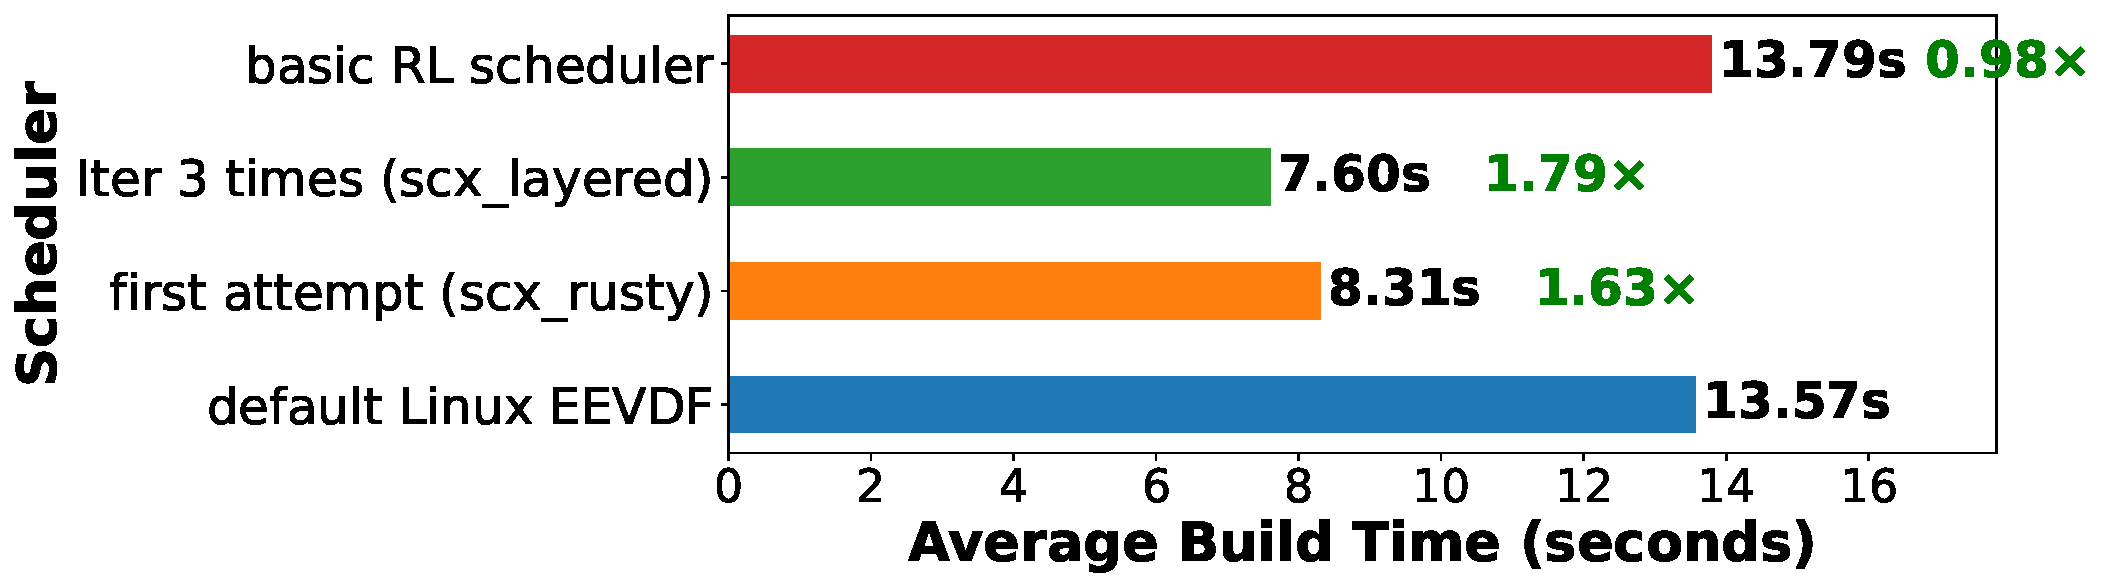
\includegraphics[width=\textwidth]{sections/Linux_build_benchmark_results.pdf}
        \caption{AI configured scheduler for Linux build time}
        \label{fig:performance-comparison}
    \end{subfigure}
    \vspace{0.3cm}
    \begin{subfigure}[b]{\textwidth}
        \centering
        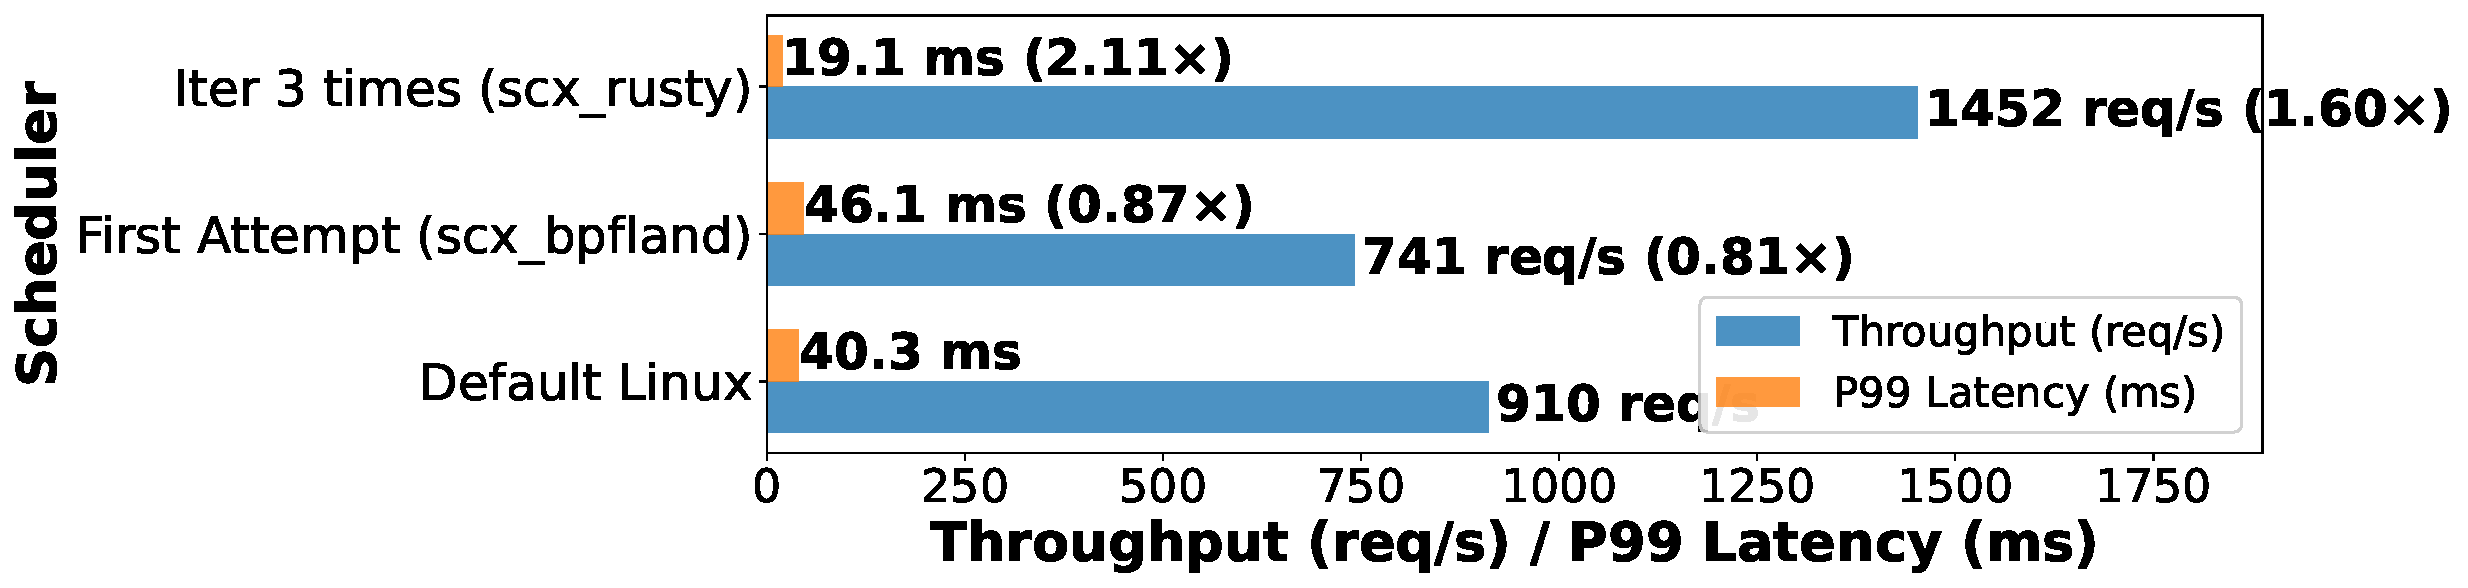
\includegraphics[width=\textwidth]{sections/schbench_performance_comparison.pdf}
        \caption{AI configured scheduler for Schbench latency and throughput}
        \label{fig:schbench-comparison}
    \end{subfigure}
\end{minipage}
\hfill
\begin{minipage}{0.48\textwidth}
    \begin{subfigure}[b]{\textwidth}
        \centering
        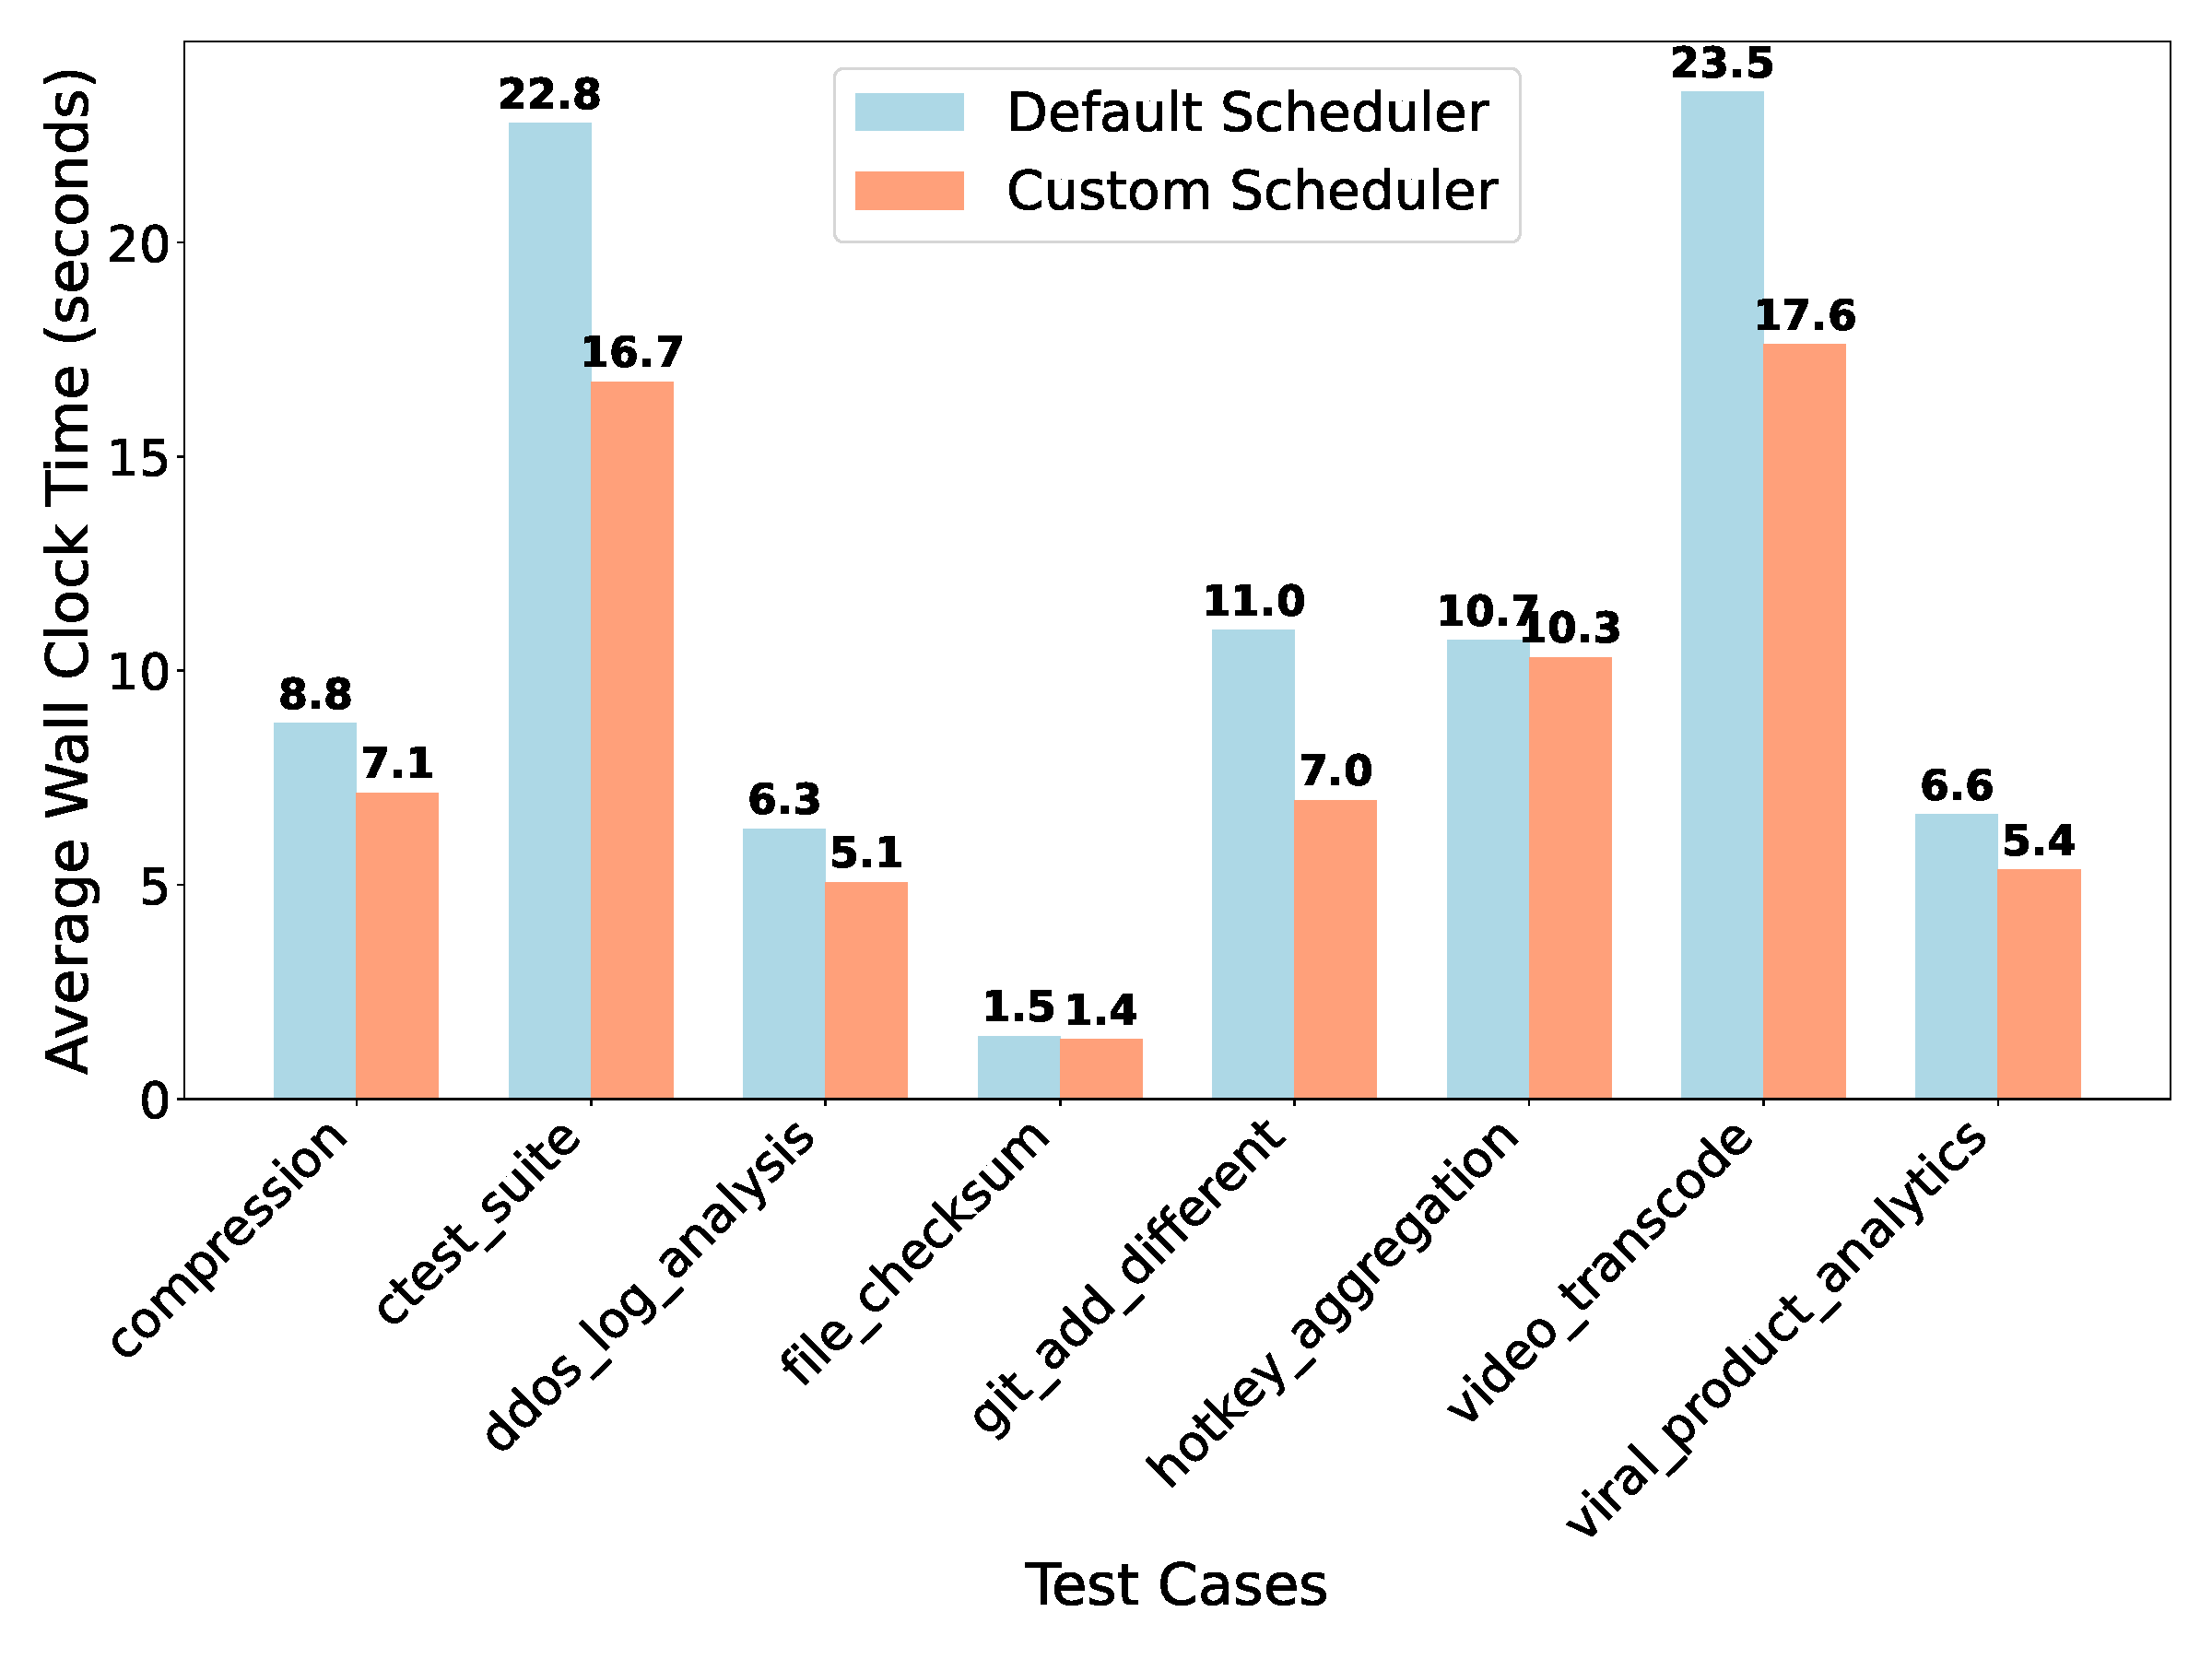
\includegraphics[width=\textwidth]{sections/scheduler_performance_comparison.pdf}
        \caption{AI-generated scheduler for batch workloads}
        \label{fig:batch-performance}
    \end{subfigure}
\end{minipage}
\caption{Performance evaluation of \sys across different workloads}
\label{fig:combined-performance}
\end{figure}


\textbf{New Scheduler Synthesis for Batch Workloads}: For 8 diverse batch workloads (e.g. file compression, video transcoding, software testing, and data analytics tasks) with long-tail distributions (40 parallel tasks: 39 short, one long), \agent correctly identified the optimization goal, workload pattern and implemented Longest Job First (LJF) scheduling, achieving 20\% average reduction in processing time (Figure~\ref{fig:batch-performance}). The cost for analysis averaged \$0.15 per workload. We note that the powerful Claude Opus agent successfully classified and analysis all 8 workloads, whereas the smaller Claude Sonnet model could not. Generation costs also improved from our initial experiments: time reduced 13× (33 to 2.5 minutes) and cost dropped from \$6 to \$0.45 per workload, demonstrating both performance gains and economic viability.


\section{Discussion}
\label{sec:discussion}

While prior ML approaches to system optimization, including learned indexes~\cite{kraska2018learned}, database tuning~\cite{marcus2019neo,vanaken2017ottertune}, and RL-based schedulers~\cite{mao2019decima,qiu2020firm,zhang2024mrsch,mao2019park}, require extensive training and lack semantic understanding to transfer across workloads, and recent LLM work focused on diagnostics~\cite{wang2024llmsys} and code generation~\cite{wei2024mapper,10.1145/3672197.3673434}, ours is the first to enable autonomous agents to design, configure, and generate kernel schedulers for end-to-end optimization. By leveraging LLM reasoning with sched\_ext and eBPF, \sys uniquely bridges the semantic gap between applications and system policy. Looking forward, extending our framework beyond schedulers to cache policies, DVFS, network configuration, and sysctl parameters presents opportunities for unified OS optimization, where cross-component decisions (CPU, memory, I/O, power) could unlock further gains through new inter-component dependency abstractions.

\bibliographystyle{plain}
\bibliography{sample-base}






\end{document}

% LLM Agents also make custom scheduling economically viable for short-lived workloads like CI/CD pipelines and batch jobs. For example, a \$0.45 generation cost is easily offset by a 20\% performance gain on a brief workload, thus democratizing expert-level system optimization for a wide range of previously unaddressable use cases.